\chapter[\hspace{0pt}模型建立与求解]{{\heiti\zihao{3}\hspace{0pt}模型建立与求解}}\label{chapter3: 模型建立与求解}
\removelofgap
\removelotgap

\section[\hspace{-2pt}问题1:颜色空间转换模型]{{\heiti\zihao{-3} \hspace{-8pt}问题1:颜色空间转换模型}}\label{section3: 问题1:颜色空间转换模型}


\subsection[\hspace{-2pt}模型建立与求解]{{\heiti\zihao{4} \hspace{-8pt}模型建立与求解}}\label{section3: 模型建立与求解}

% \noindent\textbf{优化方法与数学建模}

为求解 BT.2020 空间到显示屏 RGB 空间的最优线性映射矩阵 $M\in \mathbf{R}^{3\times 3}$ ,我们采样一组代表性 BT.2020 RGB 样本 $\{c_{i}\}_{i=1}^{N}\in [0,1]^{3}$ ,其色彩向量经过如下映射:
\begin{equation}
\begin{aligned}
  &c^{'}_{i} = M\cdot C_{i}
\end{aligned}
\end{equation}
然后分别映射至CIELab空间,并计算感知误差:
\begin{equation}
\begin{aligned}
 &L(M)=\frac{1}{N}\sum_{i=1}^{N}\Delta E_{00}(Lab(M_{BT\rightarrow XYZ} \cdot c_{i}), Lab(M_{DP\rightarrow XYZ}\cdot (M\cdot c_{i})))
\end{aligned}
\end{equation}
优化目标为:
\begin{equation}
\begin{aligned}
  &\underset {M\in \mathbb{R}^{3\times 3}}{min}L(M)
\end{aligned}
\end{equation}

为求解上述非线性、不可导且可能存在多个局部极小值的优化问题,我们引入差分进化(Differential Evolution, DE)算法。DE 是一种基于种群的全局优化方法,具有较强的鲁棒性与跳出局部最优的能力。

\noindent\textbf{(1)参数编码与搜索空间}
将 $M\in \mathbb(R^{3\times 3})$ 展开为9维向量 $\mathbf{x}\in \mathbb{R^{9}}$ ,并定义搜索空间边界为:
\begin{equation}
\begin{aligned}
  &x_{j}\in [-2,2]m\ \ j=1,...,9
\end{aligned}
\end{equation}
\noindent\textbf{(2)初始化种群}
生成 $NP$ 个个体 $\mathbf{x}_{i}^{(0)}\in \mathbb{R^{9}}$:
\begin{equation}
\begin{aligned}
  &x^{(0)}_{i,j}=l_{j}+r_{i,j}\cdot (u_{j}-l_{j}),\ \ r_{i,j}\thicksim \mathcal{U}(0,1)
\end{aligned}
\end{equation}

\noindent\textbf{(3)变异操作}
对第 $i$ 个个体,在不同个体中随机选择 $\mathbf{x}_{r1},\mathbf{x_{r2}},\mathbf{x_{r3}}$ ,构造差分向量:
\begin{equation}
\begin{aligned}
  &\mathbf{v_{i}}=\mathbf{x_{r1}}+F\cdot (\mathbf{x_{r2}}-\mathbf{x_{r3}})
\end{aligned}
\end{equation}
其中 $F\in (0,2)$ 是差分缩放因子,控制探索强度。

\noindent\textbf{(4)交叉操作}
构造试验个体 $\mathbf{u_{i}}$:
\begin{equation}
\begin{aligned}
  &u_{i,j}=
  \begin{cases}
    v_{i,j},\ \ \ rand_{j}<CR\ or\ j=j_{rand}\\
    x_{i,j}^{t},\ \ \ otherwise
  \end{cases}
\end{aligned}
\end{equation}
其中 $CR\in [0,1]$ 为交叉概率,$j_{rand}$ 确保至少一维来自 $\mathbf{v_{i}}$。

\noindent\textbf{(5)选择操作}
通过目标函数比较试验解与当前个体,选择保留更优者:
\begin{equation}
\begin{aligned}
  &\mathbf{x}_{i}^{t+1}=
  \begin{cases}
    \mathbf{u}_{i},\ \ \ L(\mathbf{u_{i}})<L(\mathbf{x^{(t)}_{i}})\\
    \mathbf{x}_{i}^{(t)},\ \ \ otherwise
  \end{cases}
\end{aligned}
\end{equation}

综上所述,为优化色彩转换矩阵 $M$,本文选用差分进化算法(DE)。该方法将 $M$ 参数化为9维向量,并在预设的搜索空间边界内进行优化。通过其经典的种群初始化、变异、交叉及选择等核心操作,DE算法能够迭代地搜寻旨在最小化以 $\Delta E_{00}$ 度量的感知色彩差异的解。鉴于目标函数的非线性、不可导以及可能存在多个局部极小值的特性,DE算法的全局优化能力和鲁棒性,使其成为获取高质量色彩映射的有效计算途径。

% \noindent\textbf{差分进化算法(Differential Evolution, DE)}

\subsection[\hspace{-2pt}问题一结果分析]{{\heiti\zihao{4} \hspace{-8pt}问题一结果分析}}\label{section4: 问题一结果分析}


为实现 BT.2020 色域向目标显示屏 RGB 色域的最优映射,本文构建了感知误差最小化的优化模型,目标为在 CIELab 空间中最小化 $\Delta E_{00}$ 感知色差。我们采样了多个 BT.2020 RGB颜色点,并通过线性映射矩阵 $M\in \mathbb{R}^{3\times 3}$ 变换后,转化至目标显示屏空间,再经过标准变换矩阵应设至 XYZ、CIELab 空间,并利用 $\Delta E_{00}$ 公式计算感知误差。

在模型求解过程中,本文采用了差分进化(Differential Evolution, DE)优化方法,对初始映射矩阵进行迭代寻优。为验证我们模型的稳定性,并提供更可靠的性能评价,我们执行了 50 轮随机优化,并统计其性能指标。主要分析结果如下:

\noindent\textbf{(1)$\Delta E_{00}$感知误差分布}

图 1 显示了在50次独立优化实验中,各次优化所达成的最终 $\Delta E_{00}$ 损失值分布情况。其中最大值为 1.0183 ,这表明映射结果在感知层面极为接近参考目标。均值为 0.0744 ,标准差为 0.2083 。这表明该基于 $\Delta E_{00}$ 损失函数的差分进化算法在不同采样条件下都能稳定收敛于较小的感知误差区域,并且具有良好的泛化性能以及良好的稳定性和鲁棒性。
\begin{figure}[h]
\centering
\captionsetup{font={small, stretch=1.312}}
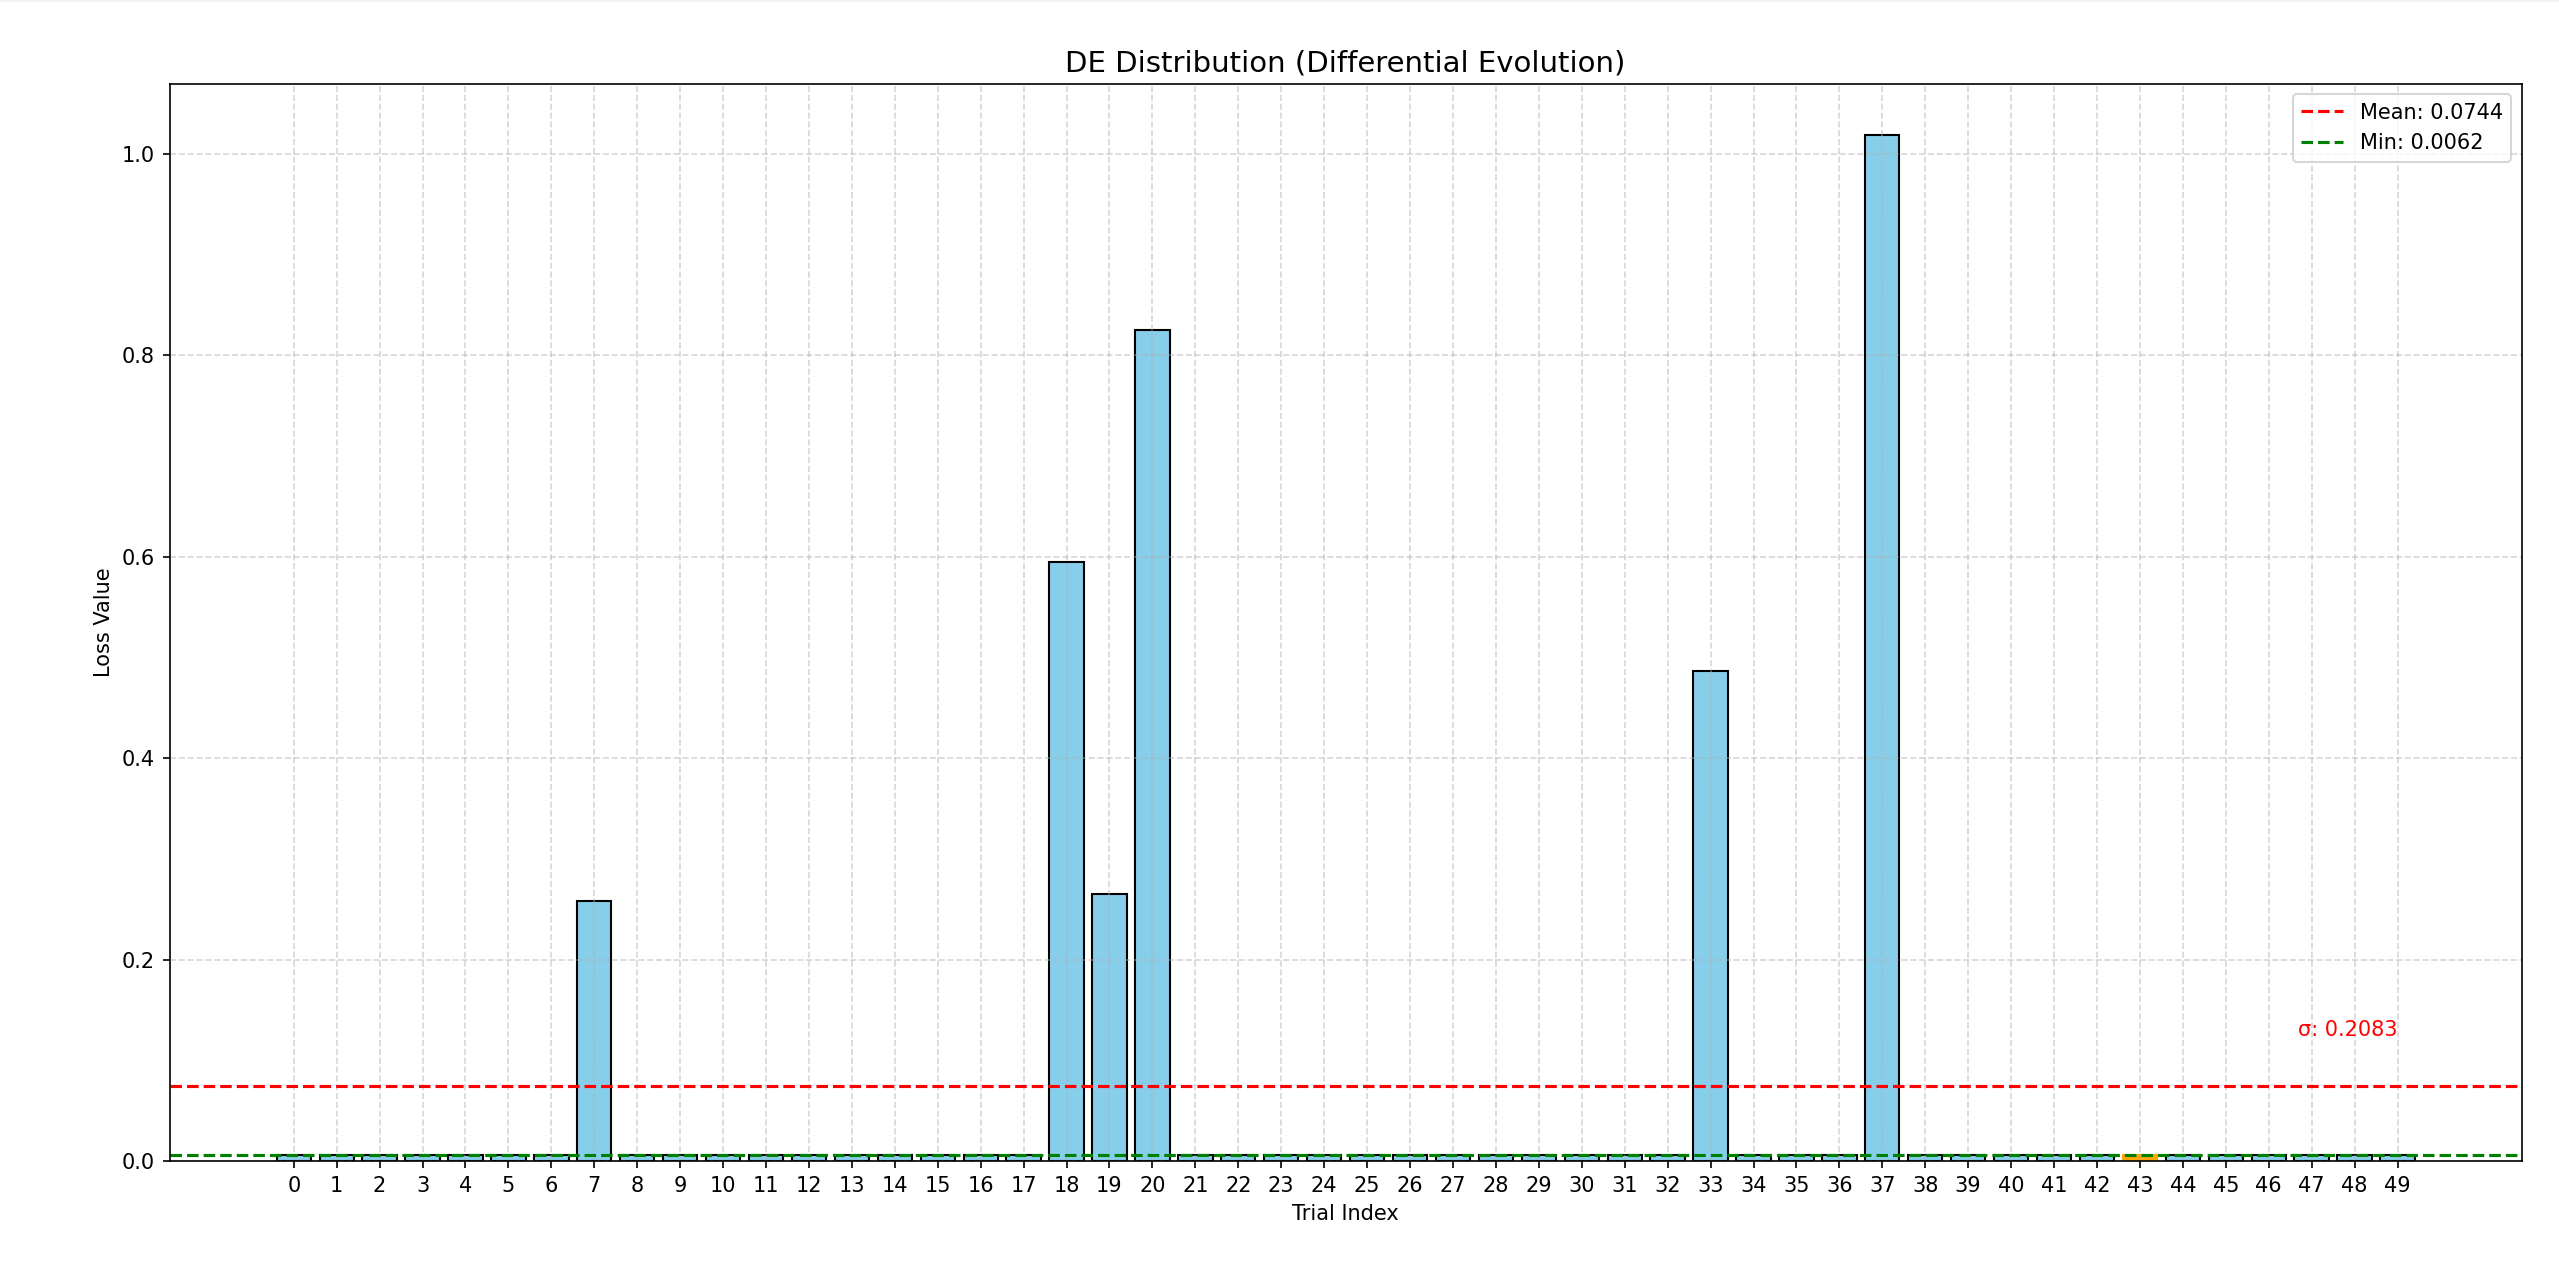
\includegraphics[width=1.0\columnwidth]{figures/DE2000.png}
% \captionsetup{justification=justified,singlelinecheck=false}
\bicaption[50次独立优化实验柱状损失图]{}[]{}
\vspace{-10pt}
\label{figure3: 柱状loss}
\end{figure}

\noindent\textbf{(2)色度空间三角形面积变化}

为评估映射后色域覆盖度变化,我们进一步对比了sRGB 色度三角与模型输出映射后所得的色度三角面积。面积通过三角形在 CIE xy 色度图上的顶点(RGB 基色经映射后的 xy 坐标)计算而得。结果表明,所有 50 次优化中,面积差绝对值均低于 0.001,说明映射后色域几乎无压缩,色彩覆盖极小损失。
\begin{figure}[htbp]
\centering
\captionsetup{font={small, stretch=1.0}}
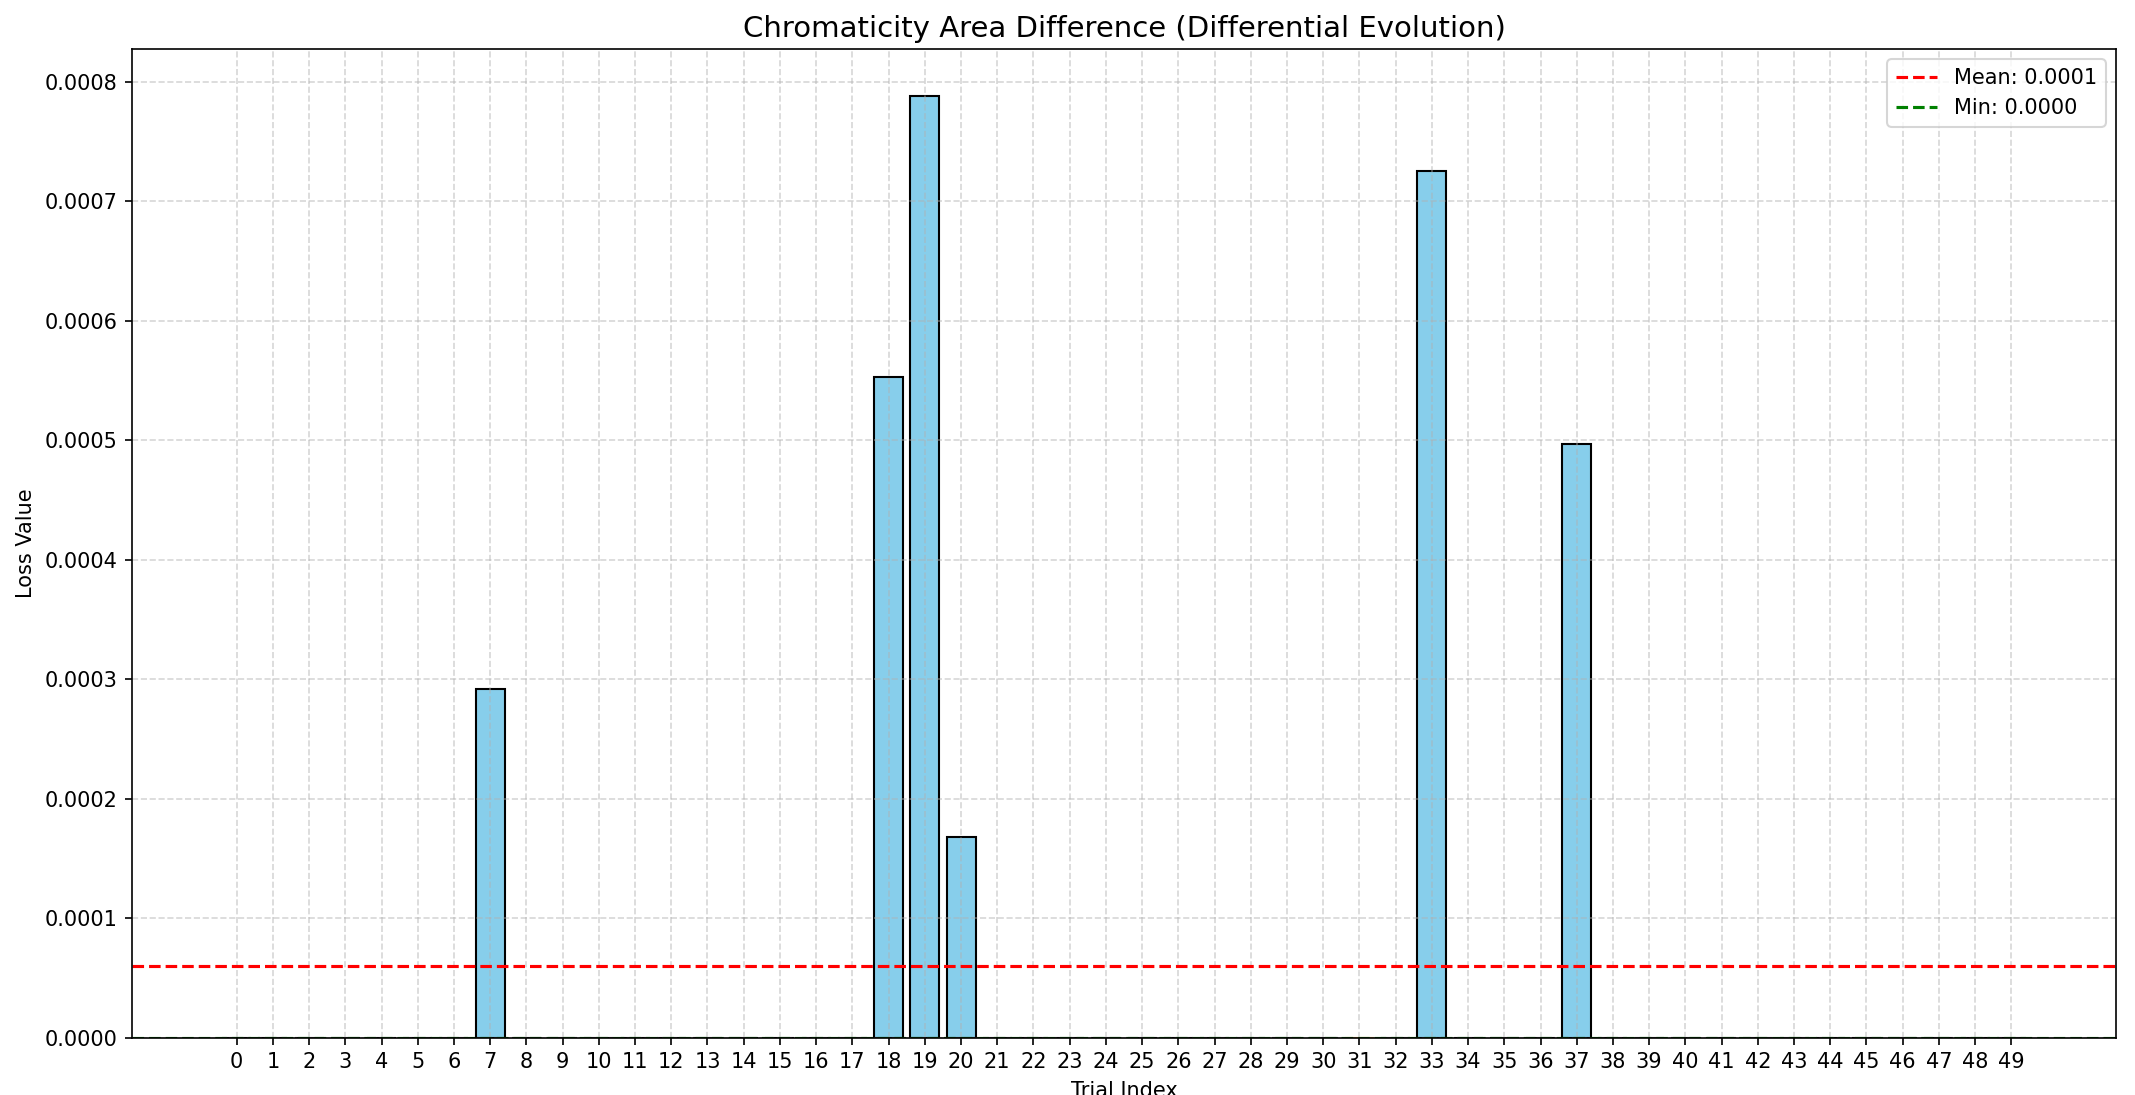
\includegraphics[width=0.8\columnwidth]{figures/面积Loss.png}
% \captionsetup{justification=justified,singlelinecheck=false}
\bicaption[50次独立优化实验面积差图]{}[]{}
\vspace{-10pt}
\label{figure3: 面积diff}
\end{figure}
显然我们可以得出,模型在保持色域范围完整性的同时,完成了精准的 RGB 空间映射,并且与 sRGB 的覆盖几乎一致,无明显压缩或扭曲现象。映射后的面积误差控制在 $10^{-3}$ 量级,说明模型不仅保持了色彩准确性,也很好地保留了 BT.2020 色域映射后的覆盖特性。

\noindent\textbf{(3)色度图可视化对比}

为直观评估映射效果,我们将 BT.2020、sRGB 以及映射后所得色度三角同时绘制于 CIE 1931 xy 色度图中(见图 3)。可以观察到,模型优化后所得色度三角与标准 sRGB 色域几乎完全重合,进一步验证了在极低感知误差下,实现了对目标色域的高保真拟合。
\begin{figure}[h]
\centering
\captionsetup{font={small, stretch=1.0}}
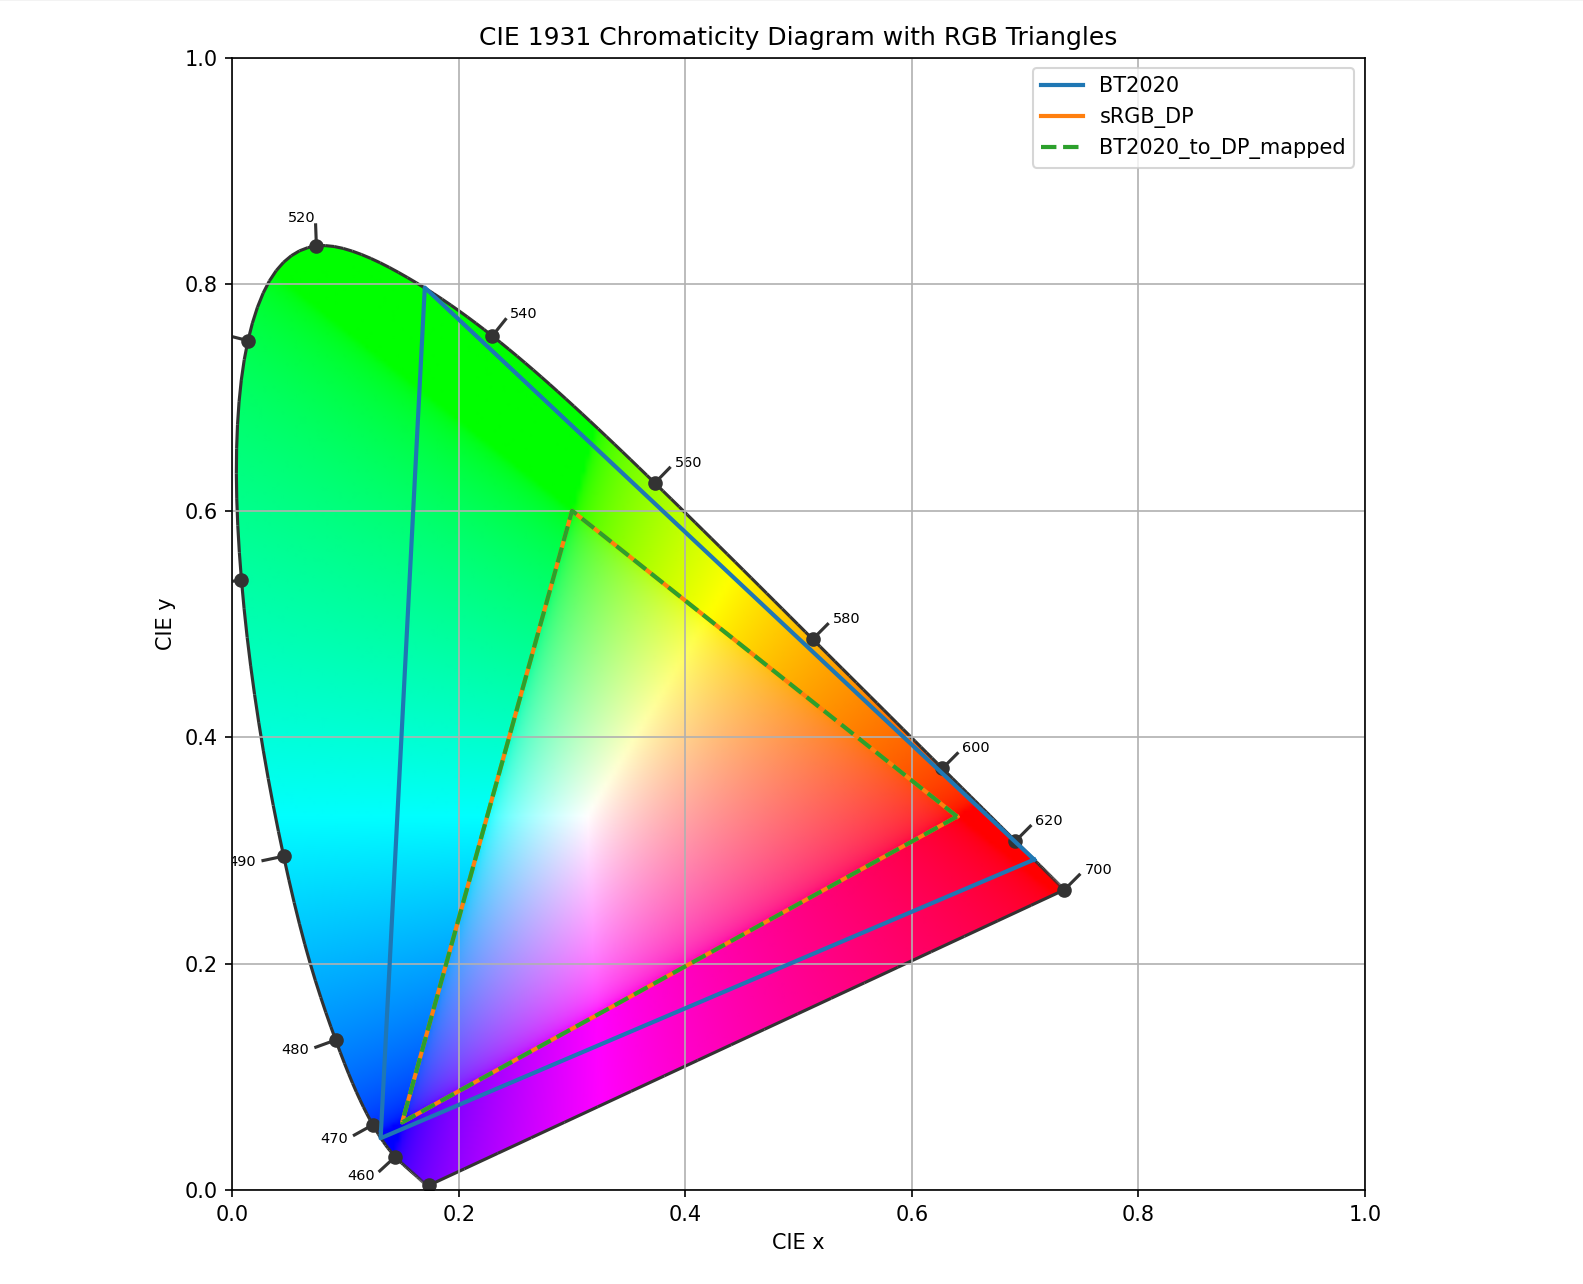
\includegraphics[width=0.8\columnwidth]{figures/色度.png}
% \captionsetup{justification=justified,singlelinecheck=false}
\bicaption[色度图]{}[]{}
\vspace{-10pt}
\label{figure3: 色度图}
\end{figure}


\section[\hspace{-2pt}问题2:四通道到五通道颜色转换模型]{{\heiti\zihao{-3} \hspace{-8pt}问题2:四通道到五通道颜色转换模型}}\label{section3: 问题2:四通道到五通道颜色转换模型}

\section[\hspace{-2pt}问题3:LED显示器颜色校正模型]{{\heiti\zihao{-3} \hspace{-8pt}问题3:LED显示器颜色校正模型}}\label{section3: 问题3:LED显示器颜色校正模型}